% !TeX root = Thesis.tex
\chapter{The Maslov Index}\label{chap:maslov}

In chapter \ref{chap:bffh} we discussed filtered Floer homology and the corresponding barcodes, though we postponed discussion of the grading of the Floer complex. This grading is based on the Maslov index of a periodic orbit of a Hamiltonian, which is the subject of this chapter. The Maslov index of a periodic orbit $x$ of $H$ is computed via the so-called Conley-Zehnder index of a certain path of symplectic matrices associated to $x$ and $H$.

There exist straightforward recipes in the literature for computing Conley-Zehnder indices of paths of symplectic matrices, see for example definition 8.1.1 in \cite{polterovich}. However, these methods fail for the paths of matrices considered in the following chapters, because they assume a finite number of transversal crossings between the path of matrices being considered and the set $Sp(2n)^0 \subseteq Sp(2n)$ of symplectic matrices with 1 as an eigenvalue, which is not the case for the piecewise linear paths we will be considering. Therefore, in this chapter we summarize the definition of the Maslov index of a periodic orbit of a Hamiltonian, as well as the definition of Conley-Zehnder index. Furthermore, we propose an alternative way to compute the Conley-Zehnder index of a path of symplectic matrices in dimension 2, which is well-adapted to concrete calculations. As an example of application, we compute the Maslov indices of critical points of an autonomous Hamiltonian.

To conclude, we relate this construction to another manner of computing CZ indices which is specialized to the two-dimensional case, due to Hofer and Kriener in \cite{hoferkriener}. [[if i relate to the one in polterovich, write here]]

\section{The General Definition}

Let $H$ be a periodic Hamiltonian with flow $\phi_t$. The Maslov index is an integer associated to a nondegenerate contractible $T$-periodic orbit $\gamma$. The process is involved, but in summary:
\begin{algorithm}[Maslov Index of a Path]\label{alg:maslovalg}
\begin{enumerate}[algorithm]
\item\label{maslovalg:step1} Since $\gamma$ is periodic, it may be seen as a smooth map $S^1 \to M$.
\item\label{maslovalg:step2} Pick a smooth map $f \colon D^2 \to M$, where $D^2$ is the disk, whose restriction to the border coincides with $\gamma$.
\item\label{maslovalg:step3} Pick smooth functions $Z_1, \dots, Z_{2n} \colon D^2 \to TM$, such that, for each $x 	\in D^2$, $\{Z_i(x)\}$ forms a symplectic basis for $T_{f(x)} M$.
\item\label{maslovalg:step4} Now that $T_{\gamma(t)} M$ has a chosen basis for each $t \in S^1$, we may write the derivative of the flow at $\gamma(0)$, i.e. the map $(\dl \phi_t)_{\gamma(0)}$, as a $2n \times 2n$ symplectic matrix, which we will call $A(t)$. Note that $A(t)$ will not be periodic.
\item\label{maslovalg:step5} Given a path of symplectic matrices, such as $A(t)$, where $A(T)$ has no eigenvalue equal to one, it is possible to associate to it an integer called the Conley-Zehnder index. Such a path is said to be \emph{non-degenerate}.
\end{enumerate}
\end{algorithm}

In turn, it is now necessary to compute the Conley-Zehnder index of a non-degenerate path of matrices $A(t)$. To do so first requires one to establish the existence of a map from the symplectic matrices to $S^1$.

\begin{theorem}\label{rhodef}
There exists a unique sequence of maps $\rho_n \colon Sp(2n) \to S^1$ (the $n$ is often omitted) which satisfies the following properties.
\begin{enumerate}[label=\roman*)]
\item If $A, T \in Sp(2n)$ then $\rho(T A T^{-1}) = \rho(A)$,
\item If $A$ and $B$ are symplectic matrices,
\begin{equation}
\rho\left(\begin{bmatrix} A & 0 \\ 0 & B \end{bmatrix}\right) = \rho(A) \rho(B),
\end{equation}
\item\label{rhodef:xy} If $A$ is a symplectic matrix of the form $A = \begin{bmatrix} X & -Y \\ Y & X \end{bmatrix}$, i.e. $A \in Sp(2n) \cap O(2n) \cong U(n)$, then
\begin{equation}
\rho(A) = \det(X + \I Y).
\end{equation}
\item\label{rhodef:realev} If all eigenvalues of $A$ are real, then
\begin{equation}
\rho(A) = (-1)^{m_0/2},
\end{equation}
where $m_0$ is the number of negative eigenvalues, counted with multiplicity,
\item $\rho(A^\transposed) = \rho(A^{-1}) = \conj{\rho(A)}$.
\end{enumerate}

Furthermore, if $A$ is a symplectic matrix whose eigenvalues are all distinct, $\rho(A)$ may be computed using the following formula
\begin{equation}\label{rhoformula}
\rho(A) = (-1)^{m_0/2} \prod \lambda^{\sign \Im \omega(\conj v, v)},
\end{equation}
where the product is taken over the eigenvalues of $A$ with positive imaginary part and unit norm, and to each such $\lambda$ we have associated  a (in general, complex) eigenvector $v$, and we have implicitly extended the 2-form $\omega$ on $\R^{2n}$ in the obvious way to $\C^{2n}$.
\end{theorem}

\begin{proof}
See \cite{audin}, Theorem 7.1.3 on page 192.
\end{proof}

We are now ready to define the Conley-Zehnder index of a non-degenerate path of symplectic matrices $A(t)$:
\begin{algorithm}[Conley-Zehnder Index of a Path of Matrices]
\begin{enumerate}[algorithm]
\item Define $Sp(2n)^*$ as the collection of symplectic matrices that do not have 1 as an eigenvalue. It is a known fact \cite[proposition~7.1.4]{audin} that $Sp(2n)^*$ is composed of two path-connected components, $Sp(2n)^+$ and $Sp(2n)^-$, labeled by the sign of $\det(A-I)$. Note that $A(T) \in Sp(2n)^*$, so it must lie in one of these two components.
\item\label{maslov:step2} Define the matrices $W^+$ and $W^-$ as
\begin{equation}
W^+ = - I, \quad W^- \mleft[\begin{array}{c|c}
\begin{matrix} 2 & 0 \\ 0 & 1/2 \end{matrix} & 0\\
\hline
0 & -I
\end{array}\mright].
\end{equation}
Note that $W^\pm \in Sp(2n)^\pm$, and so any matrix in $Sp(2n)^*$ can be connected via a path (in $Sp(2n)^*$) to either $W^+$ or $W^-$. Consequently, we extend $A(t)$ to the interval $\interval 0 {2T}$, where for $t \in \interval T {2T}$ the path $A(t)$ represents such a path connecting $A(T)$ to $W^\pm$.
\item Define $\alpha(t) = \rho(A(t))$ for $a \in \interval 0 {2T}$. By property \ref{rhodef:realev} from theorem \ref{rhodef}, $\rho(W^\pm) = \pm(-1)^n$, and also $\rho(I) = 1$. Therefore, $\rho \circ \alpha$ is a path in $S^1$ starting at $1$ and ending at $1$ or $-1$. Therefore, taking the square (viewing $S^1 \subseteq \C$) one obtains a loop $\rho^2 \circ \alpha$ starting and ending at $1$.
\item Now that we have a loop in $S^1$, we can obtain an integer by considering its winding number: the number of times the loop does a full turn around the circle. It is necessary to establish which direction is positive. Generally, one considers the counterclockwise direction to be the positive direction, but for purposes of the Conley-Zehnder index we count the number of \emph{clockwise turns}.
\end{enumerate}
\end{algorithm}
The integer resulting from the above procedure is called the Conley-Zehnder index of the path $A(t)$, denoted $\mu(A(t))$, and finally we define the Maslov index of the periodic orbit $\gamma$ above, also denoted with the symbol $\mu(\gamma)$, as the Conley-Zehnder index of the corresponding matrix path $A$.

It is a nontrivial fact that, under the assumption that the symplectic manifold $M$ is aspherical, the corresponding integer does not depend on any of the choices done in the process, only on the path and on the Hamiltonian flow. The details may be found in \cite{audin}, whose whole 7th chapter is dedicated to the definition, and well-definition, of this index.

The Conley-Zehnder index of a path of matrices is also sometimes referred to as the Maslov index of that path, such as in \cite{audin}. We will adopt this nomenclature.

\section{The Particular Case of \texorpdfstring{$Sp(2)$}{Sp(2)}}\label{sec:maslovsp2}

The theory of the Maslov index simplifies greatly in the two-dimensional case. This is partly due to the much greater control over the spectrum of a matrix. In two dimensions, the symplectic matrices coincide with those whose determinant equals one, and so their spectrum is entirely determined by their trace.

\begin{prop}\label{prop:lambdafromtau}
Let $A = \mleft[\begin{smallmatrix} a & b \\ c & d \end{smallmatrix}\mright]$ be a $2 \times 2$ symplectic matrix, that is, it satisfies the equation $ad - bc = 1$. Then, the spectrum of $A$ can be written in terms of its trace, $\tau = a+d$, as
\begin{equation}\label{lambdafromtau}
\lambda_\pm = \frac{\tau \pm \sqrt{\tau^2 - 4}}2.
\end{equation}

Consequently, the behavior of the spectrum can be qualitatively described as follows
\begin{itemize}
\item If $\tau \geq 2$, both eigenvalues are positive real numbers,
\item If $-2 \leq \tau \leq 2$, both eigenvalues lie on the unit circle as a conjugate pair,
\item If $\tau \leq -2$, both eigenvalues are negative real numbers.
\end{itemize}
\end{prop}

\begin{proof}
Equation \eqref{lambdafromtau} is a consequence of the well-known fact that the characteristic polynomial of a $2 \times 2$ matrix $A$ is $p(\lambda) = \lambda^2 - (\trace A) \lambda + \det A$.

The quantitative behavior is proved in two cases.
\begin{itemize}
\item Suppose that $\abs \tau \geq 2$. Then $\lambda_\pm$ is real. Furthermore, $\lambda_{\sign \tau}$ has the same sign as $\tau$, and since $\lambda_+ \lambda_- = 1$, both eigenvalues must have the same sign.
\item Suppose that $\abs \tau \leq 2$. Then, the square root term is purely imaginary and so the absolute value of $\lambda_\pm$ can be computed by the pythagorean theorem, being equal to 1. Since $\lambda_+ = 1/\lambda_-$, we conclude that $\lambda_+ = \conj{\lambda_-}$.
\end{itemize}
\end{proof}

\begin{corollary}\label{sp2sgn}
A matrix $A \in Sp(2)$ is in $Sp(2)^*$ iff $\trace A \neq 2$. In this case, it is in $Sp(2)^{\sign(2 - \trace A)}$.
\end{corollary}

\begin{proof}
Using the notation of proposition \ref{prop:lambdafromtau}, since $\lambda_+ \lambda_- = 1$, the only way for either eigenvalue to be equal to 1 is for both of them to be equal to 1. Therefore, if any eigenvalue is one, $\trace A = \lambda_+ + \lambda_- = 2$. On the other hand, if $\trace A = 2$, by \eqref{lambdafromtau} both eigenvalues are one.

To determine the sign of $\det(A-I)$, we compute it directly using a known formula for the characteristic polynomial
\begin{equation}
\det(A-I) = 1^2 - (\trace A) \times 1 + \det A = 2 - \trace A.
\end{equation}
\end{proof}

\begin{remark}
Note the counter-intuitive signs. If $\trace A > 2$ then $A \in Sp(2)^-$, not $Sp(2)^+$. The counter-intuitiveness extends to the $W^\pm$ matrices, given that $\rho(W^\pm) = \mp 1$.
\end{remark}

\begin{corollary}\label{sp2pm}
Let $A \in Sp(2)$. Then, $\rho(A) = 1$ iff $A \in Sp(2) \setminus Sp(2)^+$, i.e. iff $\trace A \geq 2$. Furthermore, $\rho(A) = -1$ iff $\trace A \leq -2$.
\end{corollary}

\begin{proof}
We divide the proof in three cases.
\begin{itemize}
\item If $\trace A \geq 2$, both eigenvalues of $A$ are positive, and so using property \ref{rhodef:realev} from theorem \ref{rhodef} we conclude $\rho(A) = 1$.
\item If $\trace A \leq -2$, both eigenvalues of $A$ are negative, and so for the same reason $\rho(A) = -1$.
\item If $-2 < \trace A < 2$, both eigenvalues are in $S^1 \setminus \R$. Furthermore, they are distinct, and so we may apply equation \eqref{rhoformula} to compute
\begin{equation}\label{sp2pm:3}
\rho(A) = \lambda_+^\sigma,
\end{equation}
where $\sigma$ is either $1$ or $-1$. Therefore, in this case $\rho(A)$ is either $\lambda_+$ or $\lambda_-$ and necessarily not a real number.
\end{itemize}
\end{proof}

The above propositions, notably corollary \ref{sp2pm}, greatly simplify the work of calculating the Maslov index in dimension 2, specifically in step \ref{maslov:step2}, which consists of extending the path $A(t)$ to one with endpoint in $W^\pm$.

\begin{corollary}\label{sp2rhoextension}
Let $A \in Sp(2)^*$, and define $A(t)$ as a path in $Sp(2)^*$ such that $A(0) = A$ and $A(1) = W^\pm$. Then, $\rho(A(t))$ has one of two possible behaviors:
\begin{itemize}
\item If $\rho(A) = 1$ then $\rho(A(t))$ is constant equal to one,
\item If $\rho(A) \neq 1$ then $\rho(A(t))$ is a path in $S^1 \setminus \{1\}$ with $\rho(A(1)) = -1$.
\end{itemize}
\end{corollary}

\begin{proof}
If $\rho(A) = 1$ then $A \in Sp(2)^-$ by corollary \ref{sp2pm}. Since the path connecting $A$ to $W^-$ remains in $Sp(2)^-$, and so $\rho(A(t))$ is constant equal to 1 by the same corollary.

If $\rho(A) \neq 1$ then $A \in Sp(2)^+$, and so $A(t)$ connects $A$ to $W^+$. Since this path does not leave $Sp(2)^+$ it never attains the value $1$, and $\rho(A(1)) = \rho(W^+) = -1$.
\end{proof}

Due to corollary \ref{sp2rhoextension}, the algorithm to calculate the Maslov index of a path of matrices can be simplified as follows.

\begin{prop}
Let $A(t)$ be a path of matrices in $Sp(2)$ with $A(T)$ in $Sp(2)^*$. Then, the Maslov index of the path $A(t)$ can be computed as follows:
\begin{algorithm}[Maslov Index of a Path of Matrices in $Sp(2)$]
\begin{enumerate}[algorithm]
\item Compute the path $\gamma(t) = \rho(A(t))$. 
\item If $\gamma(1) \neq 1$, extend it by connecting $\gamma(1)$ to $-1$, without passing through 1, otherwise leave it as-is. Call the resulting curve $\gamma_0$.
\item Compute the (clockwise) winding number of $\gamma_0^2$.
\end{enumerate}
\end{algorithm}
\end{prop}

To conclude this section, we present a further way to simplify the computations. The essential observations are the following.
\begin{itemize}
\item It is trivial to compute $\rho(A)$ when $\abs{\trace A} \geq 2$, as it coincides with $\sign \trace A$,
\item $\rho(A)$ is never $\pm 1$ when $\abs{\trace A} < 2$,
\item We are only interested in the winding number of $\rho^2(A(t))$,
\item And consequently, if for some $t_0, t_1$ we have $\trace A(t_0) = - \trace A(t_1) = \pm 2$ and $-2 < \trace A(t) < 2$ for $t_0 < t < t_1$, it suffices to compute $\rho(A(t))$ for a single value of $t \in \ointerval{t_0}{t_1}$, to know whether $\rho(A(t))$ crosses the circle in the clockwise or counter-clockwise direction.
\end{itemize}

\begin{prop}\label{calcmaslov0}
Let $A(t)$, $t \in \interval 0 T$ be a path of matrices with $A(0) = I$, $A(T) = W^\pm$. If $\trace A(t) > -2$ for all time, the Maslov index of $A$ is zero. Otherwise, there exists a partition of $\interval 0 T$ of the form
\begin{equation}\label{calcmaslov:ab1}
0 = a_0 < b_0 < a_1 < b_1 < a_2 < \dots < a_{N-1} < b_{N-1} < a_N = T
\end{equation}
which satisfies the properties
\begin{enumerate}
\item\label{calcmaslov:ab2} $(-1)^n \trace A(a_n) \geq 2$, \item\label{calcmaslov:ab3} $\trace A(b_n) \in \ointerval{-2}2$, \item\label{calcmaslov:ab4} Whenever $\trace A(x) \geq 2$ and $\trace A(y) \leq -2$, there exists some $b_n$ between $x$ and $y$.\end{enumerate}

For any such partition, the negative winding number of $\rho^2(A(t))$ is equal to
\begin{equation}\label{calcmaslov0:mu}
\mu(A(t)) = \sum (-1)^n \sign(A(b_n)_{12}).
\end{equation}
\end{prop}

\begin{proof}
First we do the easy part: If $\trace A(t) > -2$ for all time, the Maslov index of $A(t)$ is null.

By corollary \ref{sp2pm}, this hypothesis implies that $\rho(A(t))$ is never $-1$. Consequently, the path $\rho(A(t))$ is contractible, and therefore so is $\rho^2(A(t))$. As such, the winding number of $\rho^2(A(t))$ is zero, and so is the Maslov index.

Now, assume that $\trace A(t) \leq -2$ for some $t$. We prove that a partition \eqref{calcmaslov:ab1} satisfying \ref{calcmaslov:ab2}, \ref{calcmaslov:ab3} and \ref{calcmaslov:ab4} exists.

Let $U \subseteq \interval 0 T$ be the preimage under $\trace \circ A$ of $\ointerval{-2}\infty$, and $V$ the preimage of $\ointerval{-\infty}2$. Then, by a standard Lebesgue number lemma argument\footnote{See for example the proof of the path lifting property in pages 184 and 185 of \cite{leetopological}.}, there exists a partition 
\begin{equation}
0 = b_{-1} < b_0 < \dots < b_{N-1} < b_N = T,
\end{equation}
such that each interval $\interval{b_n}{b_{n+1}}$ is entirely contained in $U$ or $V$. By removing unnecessary points, we may suppose without loss of generality that
\begin{equation}
\interval{0}{b_0} \subseteq U, \interval{b_0}{b_1} \subseteq V, \interval{b_1}{b_2} \subseteq U, \dots,
\end{equation}
and furthermore that for each $n$ there exists some $a_n \in \ointerval{b_{n-1}}{b_{n}}$ such that $a_n \in U \setminus V$ or $a_n \in V \setminus U$. Without loss of generality pick $a_0 = 0$ and $a_N = T$. (In this step, we are assuming that $0 \neq N$, which is why the case $\forall_t \trace A(t) > -2$ must be done separately.)

We now have a sequence of numbers
\begin{equation}\label{tcineq}
0 = a_0 < b_1 < a_1 < b_2 < a_2 < \dots < a_{N-1} < b_{N-1} < a_{N} = T,
\end{equation}
which we will prove satisfies properties \ref{calcmaslov:ab2}, \ref{calcmaslov:ab3} and \ref{calcmaslov:ab4}.

\begin{itemize}
\item [\ref{calcmaslov:ab2}] Let $n$ be an even number. By hypothesis, $a_n \in U \setminus V$. Consequently, $a_n \not \in V$, i.e. $\trace A(a_n) \geq -2$. The proof is analogous for $n$ odd.

\item [\ref{calcmaslov:ab3}] For $1 \leq n \leq N-1$,
\begin{equation}
b_n \in \interval{b_{n-1}}{b_n} \cap \interval{b_n}{b_{n+1}} \subseteq U \cap V,
\end{equation}
which implies that $\trace A(b_n) \in \ointerval{-2}2$.

\item [\ref{calcmaslov:ab4}] Let $\trace A(x) \geq 2$ and $\trace A(y) \leq -2$. Then, $x \in V \setminus U$ and $y \in U \setminus V$, so they cannot both be in the same interval $\interval{b_n}{b_{n+1}}$. Therefore, there must be a value of $b_n$ (with $1 \leq n \leq N-1$) between them.
\end{itemize}

We now prove that given a partition $(a_n, b_n)$ satisfying \eqref{calcmaslov:ab1} and properties \ref{calcmaslov:ab2}, \ref{calcmaslov:ab3} and \ref{calcmaslov:ab4}, formula \eqref{calcmaslov:mu} holds.

First, observe that the winding number of $\rho^2(A(t))$ can be calculated in pieces, as the path $\rho^2 \circ A$ can be decomposed into its restriction to $\interval{a_0}{a_1}$, $\interval{a_1}{a_2}$, etc., so it suffices to calculate the winding number of $\rho^2(A(t))$ as $t$ varies from $a_n$ to $a_{n+1}$.

For the sake of argument, suppose that $n$ is even. We apply property \ref{calcmaslov:ab4} and corollary \ref{sp2pm} to observe that between $a_n$ and $b_n$ the trace of $A$ is never $-2$ or less, and consequently $\rho(A(t))$ is never $-1$. Since $S^1 \setminus \{-1\}$ is contractible, there is a homotopy between every path from $\rho(A(a_n)) = 1$ and $\rho(A(b_n)) = \exp(\pm \I \theta_n)$. Therefore, without change to the winding number of $\rho^2$, we may replace the path $\rho(A(t))$ in $\interval{a_n}{b_n}$ by a reparametrization of $\e^{\pm \I \theta}$, $\theta \in \interval 0 {\theta_n}\}$. By the same argument, the path $\rho(A(t))$ for $t \in \interval{b_n}{a_{n+1}}$ may be replaced by $\e^{\pm \I \theta}$, $\theta \in \interval{\theta_n}\pi$, and so, for $t \in \interval{a_n}{a_{n+1}}$ the path $\rho^2(A(t))$ is homotopic to $\e^{\pm 2 \I \theta}$, $\theta \in \interval 0 \pi$, with winding number $\pm 1$, where the sign is the sign of $\Im \rho(A(b_n))$.

If $n$ is odd, the previous argument works the same way, but the expression for the winding number of $\rho^2(A(t))$ has the sign swapped, i.e. it becomes $- \Im \rho(A(b_n))$. Therefore, we conclude the formula
\begin{equation}
\mu(A(t)) = -\sum (-1)^n \sign \Im \rho(A(b_n)).
\end{equation}

Note the sign swap from the definition of Maslov index. All that remains is to compute $\rho(A(b_n))$.

\begin{lemma}
Let $A$ be a $2 \times 2$ symplectic matrix with trace in $\ointerval{-2}2$. Then, $\sign \Im \rho(A) = -\sign(A_{12})$.
\end{lemma}

\begin{lemmaproof}
Let us name the entries of $A$. Suppose that
\begin{equation}
A = \begin{bmatrix} a & b\\ c & d \end{bmatrix}.
\end{equation}

We will construct a path $S(t)$ from $A$ to some $A'$ whose value of $\rho$ is known. Furthermore, we will ensure that $\trace S(t)$ is always in $\ointerval{-2}2$, so that $\rho(S(t))$ is never real and therefore the sign of $\Im \rho(S(t))$ never changes.

First, observe that $b \neq 0$, for otherwise $A$ would be lower-diagonal with eigenvalues equal to $a$ and $d$, both of which are real. However, we have seen (proposition \ref{lambdafromtau}) that if the trace of $A$ is in $\ointerval{-2}2$ then its eigenvalues cannot be real.

Now, consider the straight-line path from $A$ to the matrix with null trace given by
\begin{equation}
A_0 = \begin{bmatrix}
a & b\\
c-\frac{a+d}b a & -a
\end{bmatrix}.
\end{equation}

This path is obtained via continuously adding a multiple of the first line to the second line. This does not modify the determinant, hence the path so obtained is a path of symplectic matrices. Furthermore, the trace is interpolating linearly from $a+d \in \ointerval{-2}2$ to $0$, and so it remains in $\ointerval{-2}2$.

Since the resulting matrix $A_0$ has determinant 1, it is of the form
\begin{equation}
A_0 = \begin{bmatrix}
a & b\\
-\frac{1+a^2}b & -a
\end{bmatrix}.
\end{equation}

Furthermore, any matrix of this form has null trace and determinant equal to $1$, so any continuous deformation of $A_0$ preserves the sign of the imaginary part of $\rho$. The parameter $a$ can vary over any real value, while $b$ can only vary in $\R \setminus \{0\}$. Hence, we can find a path from $A_0$ to a matrix of the form
\begin{equation}
A' = \begin{bmatrix}
0 & \pm 1\\
\mp 1 & 0
\end{bmatrix},
\end{equation}
whose value of $\rho$ is known to be $\mp 1$ by property \ref{rhodef:xy} from theorem \ref{rhodef}. Since $\sign(b) = \pm 1$, we obtain the expected result
\begin{equation}
\sign \Im \rho(A) = - \sign(A_{12}).
\end{equation}
\end{lemmaproof}
This concludes the proof of the proposition.
\end{proof}

The previous proposition requires using a path that terminates in $W^\pm$. The following corollary shores up that weakness.

\begin{corollary}\label{calcmaslov1}
Let $A(t)$, $t \in \interval 0 T$ be a path of matrices with $A(0) = I$ and $A(T) \in Sp(2)^*$. If $\trace A(t) > -2$ for all time and $\trace A(T) > 2$, the Maslov index of $A$ is zero. Otherwise, there exists a partition of the form
\begin{equation}
0 = a_0 < b_0 < a_1 < b_1 < a_2 < \dots < a_N < b_N \leq T
\end{equation}
which satisfies the properties
\begin{enumerate}
\item $(-1)^n \trace A(a_n) \geq 2$,
\item $\trace A(b_n) \in \ointerval{-2}2$,
\item Whenever $\trace A(x) \geq 2$ and $\trace A(y) \leq -2$, there exists some $b_n$ between $x$ and $y$,
\item\label{calcmaslov:ab5} Exactly one of $\trace A(a_N)$ and $\trace A(T)$ is in $\rinterval 2 \infty$.
\end{enumerate}

For any such partition, we have the formula
\begin{equation}\label{calcmaslov:mu}
\mu(A(t)) = \sum (-1)^n \sign(A(b_n)_{12})
\end{equation}
\end{corollary}

\begin{proof}
Let $A(t)$, $t \in \interval 0 T$ be the given path of matrices, and consider an extension $\tilde A(t)$, $t \in \interval 0 {\tilde T}$, such that $\tilde A(\tilde T) = W^\pm$, with $\tilde A(t) \in Sp(2)^*$ for $t \in \interval T {\tilde T}$. We apply proposition \ref{calcmaslov0} to this new path. If $\trace A(T) > 2$ then the extension connects $A(T)$ to $W^-$, and so if $\trace A(t) > -2$ for all $t \in \interval 0 T$ we are in the conditions of the easy case of proposition \ref{calcmaslov0}. If either of these two hypotheses fail then the trace of the extension is $-2$ at some point, and so by that same proposition there is a partition
\begin{equation}
0 = a_0 < b_0 < a_1 < \dots < a_{N} < b_{N} < a_{N+1} = \tilde T.
\end{equation}

Note that, since the extension does not add any new crossings with $Sp(2)^0$, it must be the case that $a_{N} < T$.

It is tempting to throw away the last term $a_{N+1}$ to obtain the partition we seek. However, it could happen that the last term $b_N$ is greater than $T$, so we may need to perturb it, and furthermore we need to verify property \ref{calcmaslov:ab5}.

\begin{itemize}
\item Suppose that $N$ is odd, i.e. that $\trace A(a_N) \leq -2$. Since the extension does not cross $Sp(2)^0$ and $\trace A(a_{N+1}) \geq 2$, we conclude that $\trace A(T) > 2$, and furthermore that $\trace A(t) > 2$ for $t \in \interval T {\tilde T}$. As a consequence, $b_N$ is already in $\interval{a_N}T$ and requires no perturbation. It is trivial to check that properties \ref{calcmaslov:ab2}, \ref{calcmaslov:ab3} and \ref{calcmaslov:ab4} hold (they are inherited from the original partition), and the fact that $\trace A(T) > 2$ guarantees that \ref{calcmaslov:ab5} holds.

\item Suppose now that $N$ is even, i.e. that $\trace A(a_N) \geq 2$. Then, since the extension does not cross $Sp(2)^0$, we have $\trace A(T) < 2$, guaranteeing \ref{calcmaslov:ab5}. If $b_N \leq T$, it requires no perturbation and the partition obtained by throwing $a_{N+1}$ away has the desired properties. In particular, this is the case if $\trace A(T) \leq -2$, due to property \ref{calcmaslov:ab3}.

It remains to consider the case where $b_N > T$, and therefore that $\trace A(T) > -2$. In this case, change $b_N$ to equal $T$. It is straight-forward to verify that the perturbed partition satisfies the necessary properties \ref{calcmaslov:ab2} to \ref{calcmaslov:ab5}.
\end{itemize}

Note that from such a partition $a_0 < b_1 < \dots < b_N$ we can recover the partition $a_0 < b_1 < \dots < a_{N+1}$ required to apply proposition \ref{calcmaslov0} to $\tilde A(t)$, by defining $a_{N+1} = \tilde T$. Property \ref{calcmaslov:ab5} is necessary to ensure that $\trace A(a_{N+1})$ has the right sign. Applying formula \eqref{calcmaslov0:mu} we may compute the negative winding number of $\rho^2(\tilde A(t))$, and consequently the Maslov index of $A(t)$, yielding the formula \ref{calcmaslov:mu}.
\end{proof}

\section{The Autonomous Case}

Let $H$ be an autonomous Hamiltonian on a symplectic manifold $M$. In this section, we will show that a necessary condition for the time-$T$ flow $\phi_T$ to be nondegenerate Hamiltonian diffeomorphism is that $H$ is a Morse function. Furthermore. we will show that, for a given Morse function $H$, the flow $\phi_T$ is nondegenerate for small $T$ and degenerate for large $T$. To this effect, we will compute the Maslov index of the critical points of $H$ and relate them to their Morse index. Afterwards, we will repeat the procedure for the two-dimensional case, as an example of application of the methods from section \ref{sec:maslovsp2}.

\begin{definition}
We say that a Hamiltonian $H$ is degenerate if the time-one flow of $H$, denoted $\phi_1$, is a degenerate Hamiltonian diffeomorphism, i.e. if there exists some $x \in M$ such that $\phi_1(x) = x$ and $(\dl \phi_1)_x$ has an eigenvalue equal to 1.
\end{definition}

Let $x$ be a critical point of $H$, i.e. $(\dl H)_x = 0$. Then, the periodic time-$T$ orbit starting at $x$ is precisely the constant orbit. In order to compute the Maslov index of this orbit (which we will call $x$, identifying the orbit and the point), we first calculate the relevant path of matrices.

Recall algorithm \ref{alg:maslovalg} to compute the Maslov algorithm of a periodic orbit.
\begin{enumerate}[algorithm]
\item See $x$ as the constant map $S^1 \to M$ equal to $x$.
\item Extend it to the disk as the constant map.
\item Let $z_1, \dots, z_{2n}$ be a symplectic basis of $T_x M$. We define $Z_i(x) = z_i$ for $x \in D^2$.
\item We will write $(\dl \phi_t)_x$ in matricial form as $A(t)$, using the basis $z_i$ in both the domain and codomain; see theorem \ref{thm:dphimatrix} below.
\item Finally, we compute the Maslov index of $A(t)$.
\end{enumerate}

\begin{theorem}\label{thm:dphimatrix}
Let $z_1, \dots, z_{2n}$ be a symplectic basis of $T_x M$, where $x$ is a critical point of the Hamiltonian $H$. Let $A(t)$ be the matrix representing $(\dl \phi_t)_x$ in this basis, and let $S$ be the Hessian matrix of $H$ in this basis, i.e.
\begin{equation}
S_{ij} = \hessian H(z_i, z_j).
\end{equation}

Then, we have the formula
\begin{equation}
A(t) = \exp(t J_0 S),
\end{equation}
where $J_0$ is the matrix given in block notation by
\begin{equation}
J_0 = \begin{bmatrix} 0 & -I \\ I & 0 \end{bmatrix}.
\end{equation}
\end{theorem}

\begin{proof}
To begin, we extend the basis $\{z_i\}$ to a symplectic frame in a neighborhood of $x$, say $Z_1, \dots, Z_{2n}$ (not to be confused with the collection of functions $Z_i \colon D^2 \to TM$ above). With it, we may write the elements of $S$ explicitly as
\begin{equation}
S_{ij} = z_i \cdot (Z_j \cdot H).
\end{equation}

Now, let us compute the entries of $A(t)$. We may write
\begin{equation}
A(t)_{ij} = \left((\dl \phi_t) z_j \right)^i = -\omega(J z_i, (\dl \phi_t) z_j),
\end{equation}
where $J$ is the almost-complex structure satisfying $J Z_i = Z_{i+n}$ for $1 \leq i \leq n$. It is represented in coordinates by the matrix $J_0$.

Note that $A(0) = I$. We calculate the time derivative of $A(t)$:
\begin{equation}
\begin{aligned}
\diff*{A(t)_{ij}}t &= - \diff*{\omega(J z_i, (\dl \phi_t) z_j)}t\\
&= - \omega(J z_i, \diff*{(\dl \phi_t) z_j}t)\\
&= - \omega(J z_i, - \Lie_{X^H} ((\dl \phi_t) Z_j))\\
&= \omega(J z_i, [X^H,(\dl \phi_t) Z_j]_x),
\end{aligned}
\end{equation}
where $\Lie_{X^H} ((\dl \phi_t)Z_j)$ denotes the Lie derivative of $(\dl \phi_t)Z_j$ with respect to $X^H$, the vector field associated to the Hamiltonian $H$.

Now, recall the following classical formula for the exterior derivative of a one-form:
\begin{equation}
\dl \eta(X,Y) = X \cdot \eta(Y) - Y \cdot \eta(X) - \eta([X,Y]).
\end{equation}

We may solve for $\eta([X,Y])$ and apply it to $\eta = J Z_i \into \omega$, which yields (at $x$)
\begin{equation}
\omega(J z_i, [X^H, Z_j]_x) = \cancel{X^H \cdot \omega(J Z_i, ((\dl \phi_t)Z_j))} - ((\dl \phi_t) z_j) \cdot \omega(J Z_i, X^H) - \cancel{\dl(J Z_i \into \omega)(X^H, ((\dl \phi_t)Z_j))},
\end{equation}
where the first and third term cross out because, by hypothesis, $X^H = 0$ at $x$. Therefore, it remains to simplify the expression
\begin{equation}
- ((\dl \phi_t) z_j) \cdot \omega(J Z_i, X^H) = ((\dl \phi_t) z_j) \cdot \omega(X^H, J Z_i) = - ((\dl \phi_t) z_j) \cdot (\dl H)(J Z_i) = - ((\dl \phi_t) z_j) \cdot ((J Z_i) \cdot H).
\end{equation}

Now, let $(J_0)_{ij}$ be the entries of the matrix $J_0$. Recall that $J Z_i = \sum_k (J_0)_{ki} Z_k = -\sum_k (J_0)_{ik} Z_k$ and $(\dl \phi_t) z_j = \sum_\ell A(t)_{\ell j} z_\ell$ , and therefore
\begin{equation}
\begin{aligned}
- ((\dl \phi_t) z_j) \cdot ((J Z_i) \cdot H) &= \sum_{k,\ell} A(t)_{\ell j} z_\ell \cdot ((J_0)_{ik} Z_k \cdot H)\\
&= \sum_{k,\ell} A(t)_{\ell j} (J_0)_{ik} z_\ell \cdot (Z_k \cdot H)\\
&= \sum_{k,\ell} (J_0)_{ik} S_{\ell k} A(t)_{\ell j}\\
&= (J_0 S A(t))_{ij}.
\end{aligned}
\end{equation}

In conclusion, the matrix $A(t)$ satisfies the ODE
\begin{equation}
\begin{cases}
A(0) = I,\\
\diff*{A(t)}t = J_0 S A(t),
\end{cases}
\end{equation}
whose solution is known to be the matrix exponential $A(t) = \exp(t J_0 S)$. This concludes the proof.
\end{proof}

\begin{prop}\label{prop:maslovexpjs}
If $S$ is an invertible symmetric matrix and $T < \frac{2\pi}{\Norm S}$, where $\Norm S$ denotes the operator norm, the path $\exp(t J_0 S)$, $t \in \interval0T$ is nondegenerate and has Maslov index given by
\begin{equation}
\mu(\exp(t J_0 S)) = \Ind(S) - n,
\end{equation}
where $\Ind(S)$ denotes the usual Morse index, i.e. the number of negative eigenvalues of $S$.
\end{prop}

\begin{proof}
See \cite{audin}, proposition 7.2.1.
\end{proof}

\begin{corollary}\label{cor:hammorse}
If $H$ is a nondegenerate autonomous Hamiltonian on $M$, it is a Morse function.

If $H$ is a Morse function on $M$, its critical points are nondegenerate orbits for small enough period $T$; equivalently, if we set $T = 1$, the critical points of $H$ are nondegenerate orbits of $\varepsilon H$ for $\varepsilon$ small enough.
\end{corollary}

\begin{proof}
If $H$ is a nondegenerate autonomous Hamiltonian on $M$, then all of its orbits are nondegenerate, i.e. the derivative of the time-one flow has no eigenvalues equal to 1. In particular, this holds for the constant orbits, one for each critical point of $H$. Consequently, by theorem \ref{thm:dphimatrix}, if $S$ is the Hessian of $H$ at some critical point of $H$, in some symplectic basis, the matrix $\exp(T J_0 S)$ has no eigenvalues equal to 1. However, it is easy to see by taking the Taylor expansion of the exponential that if $v \in \ker(A)$ for some matrix $A$ then $\exp(A) v = v$. In other words, knowing that $\exp(T J_0 S)$ has no eigenvalue equal to 1 implies that $T J_0 S$ is invertible, and therefore that $S$ is invertible. In other words, the Hessian of $H$ at any critical point is nonegenerate, and so $H$ is a Morse function.

Now, suppose that $H$ is a Morse function on $M$. Then $H$ has finitely many critical points, say $x_1, \dots, x_n$. By proposition \ref{prop:maslovexpjs}, for $T < \min\left(\frac{2\pi}{\Norm{S_i}}\right)$ (where $S_i$ is the Hessian of $x_i$ represented in an arbitrary symplectic basis) all critical points are nondegenerate orbits.
\end{proof}

Corollary \ref{cor:hammorse} sheds light on the relation between Morse functions and nondegenerate autonomous Hamiltonians, showing that every nondegenerate autonomous Hamiltonian is a Morse function. Furthermore, for small enough periods the constant periodic orbits of a Morse function $H$ are nondegenerate, but we still need to talk about the nonconstant orbits.

\begin{prop}\label{prop:nonconstantorbits}
If $H$ is a nondegenerate autonomous Hamiltonian, all its periodic orbits are constant.

If $H$ is a Morse function, there exists $T>0$ such that all nonconstant periodic orbits have period greater than $T$. In conjunction with corollary \ref{cor:hammorse}, this shows that Morse functions are nondegenerate Hamiltonians for small enough periods.
\end{prop}

\begin{proof}
Let $H$ be a nondegenerate autonomous Hamiltonian, and let $\gamma(t)$ be a nonconstante periodic orbit starting at $x \in M$. Then, we claim that $\gamma$ is degenerate. In particular, we claim that $(\dl \phi_T)_x(\dot \gamma(0)) = \dot \gamma(0)$ (for any periodic orbit), and the fact that $\gamma$ is not constant guarantees that $\dot \gamma(0) \neq 0$ and so $(\dl \phi_T)_x$ has 1 as an eigenvalue.

The claim is proven as follows: It is known that $\gamma(t) = \gamma(t+T)$. In other words, $\gamma(t) = \phi_T(\gamma(t))$. If we take the derivative of both sides at zeros, we obtain the desired equality.

\smallskip

A proof of the second part of the proposition can be found in \cite{audin}, proposition 6.1.6. We present an alternate proof through more elementary methods.

Suppose that there exist nonconstant orbits with arbitrarily small periods, and define a sequence $x_n = \phi_{t_n} x_n$, with $t_n \to 0$. By taking a subsequence, we may assume without loss of generality that $x_n$ converges to some $x \in M$. The first step of the proof is to show that $x$ is a critical point of $H$. In other words, \emph{there is a lower bound to periods of orbits far from critical points}.

Pick a coordinate neighborhood $U$ of $x$, and pick another neighborhood $V$ which is compactly contained in $U$.

\begin{lemma}\label{lemma:phitVsubseteqU}
For $t$ smaller than some constant $T$, which depends only on $X^H$, $U$, and $V$, $\phi_t(V) \subseteq U$.
\end{lemma}

\begin{lemmaproof}
We perform this proof in coordinates. Therefore, all norms taken in the following are to be interpreted in the coordinates of $U$.

By decreasing $U$ if necessary, we may assume that $\Norm{X^H}$ is bounded by some constant $C$. Furthermore, it is a known fact from topology that any compact $\overline{V}$ contained in an open $U$ is a positive distance $d$ away from the outside of $U$. Setting $T = d/C$ proves the lemma.
\end{lemmaproof}

For large enough $n$, $x_n \in V$ and $t_n < T$, where $T$ is as in lemma \ref{lemma:phitVsubseteqU}. In this case, the entire orbit $\phi_t(x_n)$, $t \in \R$, is contained in $U$.

Now, suppose that $X^H_x$ is nonzero. Then, one of its coordinates is nonzero. Without loss of generality, we may suppose $(X^H_x)^1 > 0$. By decreasing $U$ if necessary, we may assume that $(X^H)^1 > 0$ in all of $U$. Therefore, $U$ cannot contain any periodic orbit of $X^H$, as any orbit entirely contained in $U$ will have strictly increasing first coordinate.

We conclude that small periodic orbits may only happen near a critical point $x$. Now we will show that they cannot happen there either. The idea is that near a critical point the orbits have to be moving slowly, so the only way for them to have a small period is to be turning very fast. Hence, we use bounds on the derivative of $X^H$ (i.e. on the second derivative of $H$) to show that the velocity cannot vary too much, thereby obtaining a contradiction.

In what follows, assume that $x_n$, $t_n$ and $x$ are as above, and that $U$ is a coordinate neighborhood of $x$. All computations are done in coordinates, and it is assumed that $n$ is large enough that the orbits starting at $x_n$ never leave $U$.

\begin{lemma}\label{lemma:boundsxh}
By decreasing $U$ if necessary, there exist constants $0 < c < L$ such that, for $p, q \in U$,
\begin{equation}\label{eq:boundsxh}
c \Norm{p-q} \leq \Norm{X^H_p - X^H_q} \leq L \Norm{p-q}.
\end{equation}
\end{lemma}

\begin{lemmaproof}
We begin by proving the right inequality of \eqref{eq:boundsxh}:
\begin{equation}
\Norm{X^H_p - X^H_q} = \Norm*{\int_0^1 \diff*{X^H_{q + t(p-q)}}t \dl3 t} = \Norm*{\int_0^1 (\jacobian X^H)_{q+t(p-q)} (p-q) \dl3 t} \leq \max(\Norm{\jacobian X^H}) \Norm{p-q},
\end{equation}
where the norm in the last term should be interpreted as maximum of the operator norm of the Jacobian of $X^H \colon U \to \R^{2n}$, taken over $U$. By decreasing $U$ if necessary (by replacing it with precompact set), this maximum exists. It is the $L$ in \eqref{eq:boundsxh}.

We move on to the other inequality. Again, we write
\begin{equation}
\Norm{X^H_p - X^H_q} = \Norm*{\int_0^1 (\jacobian X^H)_{q+t(p-q)} (p-q) \dl3 t}.
\end{equation}

Now, define $E(p) = (\jacobian X^H)_p - (\jacobian X^H)_x$. Again by decreasing $U$, we may suppose that $\Norm{E(p)} \leq \varepsilon$ for $\varepsilon$ of our choosing, by the continuity of the Jacobian of $X^H$. Therefore,
\begin{equation}
\begin{aligned}
\Norm{X^H_p - X^H_q} &= \Norm*{\int_0^1 (\jacobian X^H)_{q+t(p-q)} (p-q) \dl3 t}\\
&\geq \Norm*{\int_0^1 (\jacobian X^H)_{x} (p-q) \dl3 t} - \Norm*{\int_0^1 E(q + t(p-q)) (p-q) \dl3 t}\\
&\geq \Norm*{(\jacobian X^H)_{x} (p-q)} - \int_0^1 \Norm{E(q + t(p-q)) (p-q)} \dl3 t\\
&\geq \Norm*{(\jacobian X^H)_{x} (p-q)} - \varepsilon \Norm{p-q}.
\end{aligned}
\end{equation}

Now we finally use fact that $H$ is a Morse function. We will show (see lemma \ref{lemma:jacobianxh} below) that $(\jacobian X^H)_x$ is invertible. In this case,
\begin{equation}
\begin{aligned}
\Norm{X^H_p - X^H_q} &\geq \Norm*{(\jacobian X^H)_{x} (p-q)} - \varepsilon \Norm{p-q}\\
&\geq \left( \frac1{\Norm{(\jacobian X^H)_x^{-1})}} - \varepsilon \right) \Norm{p-q},
\end{aligned}
\end{equation}
hence for small enough $\varepsilon$ (so, by picking small enough $U$), there exists a positive constant $c$ such that $\Norm{X^H_p - X^H_q} \geq c \Norm{p-q}$.
\end{lemmaproof}

\begin{lemma}\label{lemma:jacobianxh}
Let $U$ be a coordinate neighborhood of $x$, a critical point of the Morse function $H$. Let $\Omega$ be the matrix representation of the symplectic form $\omega$ in coordinates, i.e. $\Omega_{ij} = \omega(\partial_i, \partial_j)$. Recall that the nondegeneracy of the symplectic form implies that $\Omega$ is invertible. Then, the Jacobian of $X^H$ at $x$, seen as a function $U \to \R^n$ is given by
\begin{equation}
(\jacobian X^H)_x = - \Omega^{-1} S,
\end{equation}
where $S$ is the Hessian of $H$.

In particular, $(\jacobian X^H)_x$ is invertible.
\end{lemma}

\begin{lemmaproof}
The proof of this lemma is simple computation. We begin by recalling the definition of $X^H$ as a function of $\omega$ and $H$:
\begin{equation}
X^H \into \omega = - \dl H,
\end{equation}
which in coordinates becomes
\begin{equation}
\sum_i (X^H)_i \Omega_{ij} = - \partial_j H.
\end{equation}

In other words, $- (\dl H)^\transposed = \Omega X^H$, hence
\begin{equation}\label{eq:xhincoords}
X^H = - \Omega^{-1} (\dl H)^\transposed.
\end{equation}

Now, we take the Jacobian at $x$. The right-hand side of \eqref{eq:xhincoords} is a product, so in principle we should use the rule for the derivative of a product, but fortunately $x$ is a critical point of $H$. Consequently, $(\dl H)_x = 0$, and so all the terms with derivatives of $\Omega^{-1}$ are null. Hence,
\begin{equation}
\jacobian X^H = - \Omega^{-1} (\jacobian (\dl H)^\transposed) = - \Omega^{-1} S,
\end{equation}
with $S$ the Hessian matrix of $H$ at $x$.
\end{lemmaproof}

With lemma \ref{lemma:boundsxh} we are finally in a position to complete the proof, by showing that for large $n$ the orbits $\phi_t(x_n)$ cannot curve too much. We begin with the bound:
\begin{equation}\label{eq:normxh1}
\Norm{X^H_{x_n} - X^H_{\phi_t(x_n)}} \leq L \Norm{x_n - \phi_t(x_n)} \leq L t_n \max(\Norm{X^H}),
\end{equation}
where the maximum is taken over the points of the orbit starting at $x_n$. Note that we implicitly assumed $0 \leq t < t_n$; this can be done without loss of generality by periodicity. If $\tau$ is the time that maximizes $\Norm{X^H}$, we obtain
\begin{equation}\label{eq:normxh2}
\max(\Norm{X^H}) = \Norm{X^H_{\phi_\tau(x)}} \leq \Norm{X^H_{x_n}} + \Norm{X^H_{\phi_\tau(x)} - X^H_{x_n}} \leq L \Norm{x_n - x} + L t_n \max(\Norm{X^H}),
\end{equation}
and so, for $n$ large such that $L t_n < 1/2$, joining \eqref{eq:normxh1} and \eqref{eq:normxh2} we obtain
\begin{equation}
\Norm{X^H_{x_n} - X^H_{\phi_t(x_n)}} \leq 2 L^2 t_n \Norm{x_n - x}.
\end{equation}

Now, let us use the lower bound from \eqref{eq:boundsxh}. With it, we conclude that
\begin{equation}
c \Norm{x_n - x} \leq \Norm{X^H_{x_n}},
\end{equation}
and therefore, for large $n$,
\begin{equation}
\Norm{X^H_{x_n} - X^H_{\phi_t(x_n)}} \leq \frac{2 L^2 t_n}c \Norm{X^H_{x_n}}.
\end{equation}

This proves that for large $n$, the velocity in the orbit $\phi_t(x_n)$ does not vary by at most a factor of $\frac{2 L^2 t_n}c$ of its original value. If this value is picked small enough, let us say smaller than a half, then the velocity of $\phi_t(x_n)$ will always be pointing roughly in the same direction as $X^H_{x_n}$, and therefore does not have enough room to turn around (within the coordinate neighborhood) and be periodic. This is the contradiction that was being sought, which proves that there are no orbits of arbitrarily small period. This completes the proof.

To make the preceding paragraph more rigorous, one may consider the periodic function $f(t) = \braket{\phi_t(x_n), X^H_{x_n}}$. For large enough $n$ as in the previous paragraph one can show $f'(t) > 0$ for all $t$, which contradicts the periodicity of $f$.
\end{proof}

\section{The Two-Dimensional Case}\label{sec:twodimensionalcase}

We will now use the tools developed in section \ref{sec:maslovsp2} to recompute the Maslov index of the critical points of a Morse function $H$.

We have already shown that a path of matrices $A(t)$ associated to such a critical point is given by
\begin{equation}
A(t) = \exp(t J_0 S), t \in \interval 0 T,
\end{equation}
with $S = \hessian H(x)$ in some symplectic basis $\{Z_i\}$, i.e. $S_{ij} = \hessian H(x)(Z_i, Z_j) = Z_i \cdot (Z_j \cdot H)$. Therefore, we investigate when such a path of matrices is nondegenerate and compute its Maslov index.

It is fortunate that the theory greatly simplifies in the two-dimensional case, allowing us to do the computations by hand.

\begin{prop}\label{prop:sidentities}
Let $S$ be a $2 \times 2$ symmetric matrix, and let $\Delta = \det S$. Then, the following identities hold.
\begin{gather}
J_0 S J_0 S = - \Delta I, \label{eq:j0sj0s}\\
\exp(t J_0 S) = \begin{cases}
\cos(\sqrt{\Delta} t) I + \frac1{\sqrt{\Delta}} \sin(\sqrt{\Delta} t) J_0 S, & \Delta > 0,\\
I + t J_0 S, & \Delta = 0,\\
\cosh(\sqrt{-\Delta} t) I + \frac1{\sqrt{-\Delta}} \sinh(\sqrt{-\Delta} t) J_0 S, & \Delta < 0.
\end{cases} \label{eq:exptj0s}
\end{gather}
\end{prop}

\begin{proof}
The proof of \eqref{eq:j0sj0s} is a simple computation. Using \eqref{eq:j0sj0s}, the identity \eqref{eq:exptj0s} can be obtained by expanding the Taylor series of the exponential and grouping terms as follows
\begin{equation}
\begin{aligned}
\exp(t J_0 S) &= 
I \color{black!60} + t J_0 S \color{black} + \frac12 t^2 (J_0 S)^2 \color{black!60} +\frac1{3!} t^3 (J_0 S)^3 \color{black} \cdots \\
&= 
I \color{black!60} + t J_0 S \color{black} - \frac12 t^2 \Delta I \color{black!60} -\frac1{3!} t^3 \Delta J_0 S \color{black} \cdots
\end{aligned}
\end{equation}

Equation \eqref{eq:exptj0s} should now be evident: the black terms correspond to cosines or hyperbolic cosines and the gray terms correspond to sines or hyperbolic sines.
\end{proof}

Proposition \ref{prop:sidentities} gives us full knowledge about $\exp(t J_0 S)$ for $S = \hessian H(x)$, and so we may use it to compute the Maslov index of this path.

\begin{prop}\label{maslovmorse}
Let $H$ be a Morse function and $x$ a critical point of $H$. Let $S = \hessian H(x)$. Then, the Maslov index $\mu(x)$ of the (constant) periodic orbit $x$ depends on the following way on the Morse index of $S$ and on the period $T > 0$:
\begin{itemize}
\item If $\Ind S = 1$ then $\mu(x) = 0$,
\item If $\Ind S = 1 \pm 1$ then the periodic orbit is nondegenerate if and only if $T \not \in \frac{2 \pi}{\sqrt\Delta} \Z$. In this case, the Maslov index is $\pm(2N+1)$, where
\begin{equation}
T \in \ointerval{\frac{2\pi}{\sqrt\Delta}N}{\frac{2\pi}{\sqrt\Delta}(N+1)}.
\end{equation}

Diagramatically, this can be represented as
\begin{figure}[H]
\centering
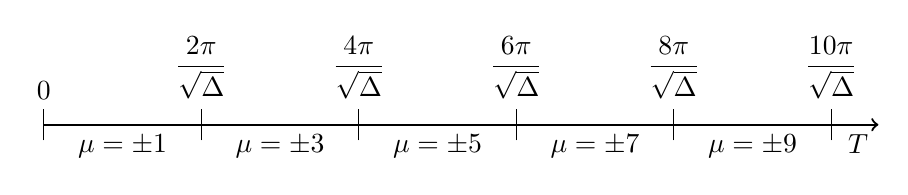
\begin{tikzpicture}
\draw[->,thick] (0,0)--(10.6,0) node[below left] {$T$};
\draw[] (0,-0.200)--(0,0.200) node[above] {0};
\foreach \i in {2,4,...,10}
\draw[] (\i,-0.200)--(\i,0.200) node[above] {$\displaystyle \frac{\i\pi}{\sqrt\Delta}$};


\foreach \i in {1,3,...,9}
\draw[] (\i,0) node[below] {$\mu = \pm \i$};
\end{tikzpicture}
\caption{Representation of the Conley-Zehnder index of the path $\exp(t J_0 S)$, $t \in \interval 0 T$ as a function of $T > 0$.}
\end{figure}
\end{itemize}
\end{prop}

\begin{proof}
We begin by solving the case $\Ind S = 1$. By inspection of equation \eqref{eq:exptj0s}, if $\Ind S = 1$ then both eigenvalues have distinct signs and $\det S = \Delta < 0$. Therefore, by \eqref{eq:exptj0s},
\begin{equation}
\trace \exp(t J_0 S) = 2 \cosh(\sqrt{-\Delta} t) \geq 2,
\end{equation}
where we used the fact that $\trace(J_0 S) = 0$. Application of corollary \ref{calcmaslov1} yields that, in this case, $\mu(x) = 0$.

We now focus on the case $\Ind S = 1 \pm 1$. In this case, by a similar calculation we obtain $\Delta > 0$ and therefore
\begin{equation}
\trace \exp(t J_0 S) = 2 \cos(\sqrt\Delta t).
\end{equation}

Therefore, by corollary \ref{sp2sgn} the path $\exp(t J_0 S)$ is degenerate iff $\cos(\sqrt \Delta T) = 1$, which happens iff $\sqrt\Delta T \in 2 \pi \Z$. This completes the proof of nondegeneracy.

\smallskip

To compute the Maslov index, we apply corollary \ref{calcmaslov1}. Since we have full knowledge of $\trace \exp(t J_0 S)$, we may build the partition required by corollary \ref{calcmaslov1} explicitly. The interval $\interval 0 T$ can be divided into intervals of size $\frac\pi{\sqrt\Delta}$, on the extrema of which the trace is $\pm 2$. Therefore, we set $a_n = n \frac\pi{\sqrt\Delta}$. We may pick any $b_n$ between $a_n$ and $a_{n+1}$; for example their midpoints, on which the trace is zero. This ensures that properties \ref{calcmaslov:ab2} and \ref{calcmaslov:ab3} hold.

Note that (for all $T$ such that our path is non-degenerate) we have $\trace \exp(t J_0 S) \in \rinterval{-2}2$, so that in order to verify property \ref{calcmaslov:ab5} the last element of our sequence $a_n$ needs to satisfy $\trace \exp(a J_0 S) = 2$, and so we terminate our sequence at $a_{2N}$, even if $a_{2N+1}$ happens to be less than $T$. Finally, we pick $b_{2N}$ arbitrarily, as long as it is between $a_{2N}$ and $\min(T, a_{2N+1})$.

In summary, we consider the partition
\begin{equation}\label{autmaslov:thepartition}
\begin{array}{c|c|c|c|c|c|c|c}
a_0 & b_0 & a_1 & b_1
& \cdots &
b_{2N-1} & a_{2N} & b_{2N} \\
\hline
0 & \frac12 \frac{\pi}{\sqrt\Delta} & \frac{\pi}{\sqrt\Delta} & \frac32 \frac{\pi}{\sqrt\Delta}
& \cdots &
\frac{2(2N-1)+1}2 \frac{\pi}{\sqrt\Delta} & 2N \frac{\pi}{\sqrt\Delta} & b_{2N}
\end{array}
\end{equation}

We have already verified most of the conditions of corollary \ref{calcmaslov1}, the only one remaining being property \ref{calcmaslov:ab4}, i.e. that whenever $\trace A(x) \geq 2$ and $\trace A(y) \leq -2$ there exists some $b_n$ between $x$ and $y$. This property is verified directly by checking that in this event $x$ is $a_n$ for some even $n$ and $y$ is $a_n$ for some odd $n$, and by construction there is always a $b_n$ between such numbers.

Corollary \ref{calcmaslov1} now tells us that the Maslov index of $A(t) = \exp(t J_0 S)$ equals
\begin{equation}
\mu(A(t)) = \sum_{n = 0}^{2N} (-1)^n \sign(A(b_n)_{12}).
\end{equation}

We compute $A(b_n)$, for $n < 2N$ explicitly as
\begin{equation}
A(b_n) = \frac1{\sqrt\Delta} \sin\left( \sqrt\Delta \frac{2n + 1}2 \frac\pi{\sqrt\Delta} \right) J_0 S = \frac1{\sqrt\Delta} (-1)^n J_0 S,
\end{equation}
and therefore $\sign(A(b_n)_{12}) = (-1)^n \sign((J_0 S)_{12})$. The case $n = 2N$ requires a little extra consideration, but it can be verified that the conclusion is the same, and so we have the identity
\begin{equation}
\mu(A(t)) = (2N+1) \sign((J_0 S)_{12}),
\end{equation}
and so it remains to relate the sign of $(J_0 S)_{12}$ to the index of $S$.

First, we make the trivial observation that $(J_0 S)_{12} = - S_{22}$, so it suffices to relate the sign of $S_{22}$ to the index of $S$.

Furthermore, observe that $S_{22}$ and $S_{11}$ have the same sign, as
\begin{equation}
S_{11} S_{22} = \Delta + S_{12}^2 > 0.
\end{equation}

Finally, this sign coincides with the sign of both eigenvalues of $S$ (which have the same sign because $\lambda_1 \lambda_2 = \Delta > 0$), and both of these signs equal the sign of the trace of $S$. In conclusion,
\begin{itemize}
\item The sign of $S_{22}$ equals the sign of the trace of $S$, which equals the sign of both eigenvalues of $S$.
\item Consequently, if $\Ind S = 0$ then these eigenvalues are positive, and therefore so is $S_{22}$ and therefore $(J_0 S)_{12} < 0$ and $\mu(A(t)) = -(2N+1)$.
\item On the other hand, if $\Ind S = 2$ then these eigenvalues are both negative, and by the same argument $\mu(A(t)) = 2N+1$.
\end{itemize}

The proof is therefore complete.
\end{proof}

We note that the usual result on small multiples of Morse functions can be recovered.

\begin{corollary}\label{cor:orbitsepsH}
Let $H$ be an autonomous Morse function on a 2-dimensional compact symplectic manifold $M$. Then, for small enough $\varepsilon > 0$, the function $\varepsilon H$ is a nondegenerate Hamiltonian, i.e. the time-one flow of $\varepsilon H$ is a nondegenerate Hamiltonian diffeomorphism. More precisely, the only periodic (time-one) orbits of $\varepsilon H$ are constants equal to critical points of $H$. In this case, the action functional of these constant orbits coincides with their value of $\varepsilon H$, and their Maslov index and Morse index are related by the formula
\begin{equation}
\mu(x) = \Ind(x) - 1.
\end{equation}
\end{corollary}

\begin{proof}
For the fact that for small $\varepsilon$ the only time-one orbits of $\varepsilon H$ are the constants, proposition \ref{prop:nonconstantorbits}.

Assume now that $\varepsilon$ is small enough that the only time-one orbits of $\varepsilon H$ are constants. Recall the definition of the action functional on a periodic orbit $x$,
\begin{equation}
\AA_{\varepsilon H}(x) = - \int_D \omega + \int_0^1 \varepsilon H(x(t)) \dl t,
\end{equation}
where $D$ is any map from the disk to $M$ whose border is $x$.

Since $x$ is constant, we might as well take $D$ to be the constant map. This makes the pullback of $\omega$ to the disk be null, and so the first term from the action functional vanishes. As for the second term, since $H$ is autonomous and $x$ is constant, we obtain simply
\begin{equation}
\AA_{\varepsilon H}(x) = \varepsilon H(x).
\end{equation}

Finally we show that, possibly by decreasing $\varepsilon$, the Maslov index of these constant orbits coincides up to a shift by one with their Morse index.

Application of proposition \ref{maslovmorse} will show that in order for the relation $\mu(x) = \Ind(x) - 1$ to be verified it suffices that for every critical point $x$ of $H$ there exists a symplectic basis for $T_x M$ such that the determinant of the Hessian of $\varepsilon H$ in that basis\footnote{It is a trivial observation, yet unnecessary for our purposes, that the determinant of the Hessian of a smooth function is independent of the symplectic basis chosen.} is less than $4 \pi^2$. In other words, it suffices that
\begin{equation}
\varepsilon < \min \left( \frac{2\pi}{\sqrt{\det \hessian H(x)}}\right),
\end{equation}
where the minimum ranges over the critical points of $H$.
\end{proof}

A somewhat surprising corollary of proposition \ref{maslovmorse} is that the Maslov indices of critical points of autonomous Hamiltonians may only take odd values or zero. As a consequence of this and the fact that Floer homology must coincide with Morse homology, if any critical point of $H$ has Maslov index different from $-1$, $0$, and $1$, then the time-one flow of $H$ must be degenerate. This allows us to prove the existence of orbits with almost all possible non-small periods.

\begin{corollary}
Let $H$ be a Morse function on the two-dimensional compact symplectic manifold $M$. Let $x_1, \dots, x_N$ be the critical points of $H$ \emph{with Morse index different from $0$}, i.e. the local maxima and minima.

For each $i = 1, \dots, N$, define $\Delta_i = \det \hessian H(x_i)$, where the determinant is taken in an arbitrary symplectic basis of $T_{x_i} M$, set $q_i = \frac{2\pi}{\sqrt{\Delta_i}}$, and $q_{\min} = \min q_i$. Then, for all $p \geq q_{\min}$, the time-$p$ flow of $H$ is a degenerate Hamiltonian diffeomorphism; equivalently, $p H$ is a degenerate Hamiltonian.

Furthermore, if we let
\begin{equation}
A = \ointerval{q_{\min}}{\infty} \setminus \bigcup q_i \Z,
\end{equation}
then for all $p \in A$ there exists a time-$p$ nonconstant periodic orbit of $H$, though $p$ may in general not be a primitive period.

[Should be able to prove that there exist orbits with periods greater than some $T$ constructed from the $\Delta_i$.]
\end{corollary}

\begin{proof}
Consider the Hamiltonian $p H$, $p > 0$. It has the same critical points as $H$, with the same indices, and the determinants of the Hessians of the $x_i$ are given by
\begin{equation}
\det \hessian(pH)(x_i) = p^2 \Delta_i.
\end{equation}

We conclude from proposition \ref{maslovmorse} that if $p \geq \frac{2\pi}{\sqrt{\Delta_i}} = q_i$ then either the critical point $x_i$ is degenerate (in the Floer sense) or or it has Maslov index in $\Z \setminus \{-1,0,1\}$. Therefore, if $p \geq q_{\min}$ either some critical point is degenerate (in which case the Hamiltonian $pH$ is degenerate) or some critical point has Maslov index in $\Z \setminus \{-1,0,1\}$. We will now show that the latter also implies that $pH$ is degenerate.

Assume for the sake of argument that $pH$ is a nondegenerate autonomous Hamiltonian which has a critical point $x$ with Maslov index $\mu(x) = m \not \in \{-1,0,1\}$. Then, the Floer complex is nontrivial at degree $m$, i.e. $\CF_m(pH) \neq \{0\}$. Therefore, since the Morse homology agrees with Floer homology, the boundary maps $\partial_m$ and $\partial_{k+1}$ must satisfy $\ker(\partial_m) = \image(\partial_{k+1})$. However, proposition \ref{maslovmorse} implies that no critical point can have Maslov index equal to $m \pm 1$, and therefore that $\CF_{m\pm1}(pH) = \{0\}$. As a consequence, $\ker(\partial_m) = \CF_m(pH)$ and $\image(\partial_{k+1}) = \{0\}$, hence $\HF_m(pH) = \CF_m(pH) \neq \{0\}$. This is a contradiction, because the Morse homology at index $m+1$ is necessarily null, as Morse indices may only take the values $0$, $1$, and $2$. This shows that $pH$ is necessarily degenerate for $p \geq q_{\min}$.

\smallskip

We now turn to showing that if $p \in A$ then there necessarily exists a $p$-periodic orbit of $H$. Indeed, as we have seen, if $p \in A$ then the Hamiltonian $pH$ is degenerate. However, if $p$ is not a multiple of $q_i$ for any $i$, then by proposition \ref{maslovmorse} every critical point of $H$ is a nondegenerate orbit. Therefore, there must be a degenerate time-one orbit of $pH$ which is not a constant, or, in other words, a non-constant time-$p$ orbit of $H$.
\end{proof}

\section{Relation to a construction by Hofer and Kriener}\label{sec:hoferkriener}

There is another construction of the Conley-Zehnder index, also specific to the 2-dimensional case, due to Hofer and Kriener. The original work can be found in section 3 of \cite{hoferkriener}, and a summary can be found in the appendix of \cite{hwz}. For convenience, we reproduce the construction.

Let $A(t)$, $t \in \interval 0 T$, be the path of $2 \times 2$ symplectic matrices whose Maslov index we intend to compute. Given a nonzero complex number $z \in \C \cong \R^2$. we can consider the path of nonzero complex numbers given by $z(t) = A(t) z$. We may write this path in polar coordinates as
\begin{equation}
z(t) = \abs{z(t)} \exp(\I \theta(t)),
\end{equation}
where $\theta(t)$ is chosen to be continuous. Then, we define the winding of $z$ by
\begin{equation}
\Delta(z) = \theta(T) - \theta(0).
\end{equation}

Finally, we define the winding interval of $A(t)$ as
\begin{equation}
I(A) = \{\, \Delta(z) \mid z \in \C \setminus \{0\} \,\}.
\end{equation}

It will be shown that this set is a closed interval of length strictly less than $\pi$, and therefore it contains at most one multiple of $2\pi$. Then, we may define the CZ index \textit{a la} Hofer and Kriener as
\begin{equation}\label{def:muhk}
\muhk(A) = \begin{cases}
2 k, & 2 k \pi \in I(A),\\
2k+1, & I(A) \subseteq \ointerval {2k\pi}{2(k+1)\pi}.
\end{cases} 
\end{equation}

We begin by verifying the statements made above, in order to ensure that $\muhk$ is well-defined.

Recall that the function $f(t) = \exp(\I t)$ is a covering map $\R \xrightarrow{f} S^1$. Therefore, the following proposition guarantees that for each $z$ a continuous argument for $z(t)$ can be found.

\begin{prop}[Path Lifting Property]\label{prop:pathliftingproperty}
Let $p \colon E \to B$ be a covering map and $\gamma \colon \interval01 \to B$ a curve. Then, for every $e \in p^{-1}(\gamma(0))$ there exists a unique continuous lift $\tilde \gamma \colon \interval01 \to E$ satisfying $\gamma = p \circ \tilde \gamma$.
\end{prop}

\begin{proof}
See proposition 11.10 in \cite{leetopological}.
\end{proof}

\begin{corollary}
Any continuous path $z(t)$ of nonzero complex numbers has a continuous argument. For any such choice, the winding of $z(t)$ is the same.
\end{corollary}

\begin{proof}
To obtain the existence of a continuous argument, apply the path lifting property to the function $t \mapsto \frac{z(t)}{\abs{z(t)}}$, using the covering map $\exp(\I\,\cdot\,) \colon \R \to S^1$ and any value of $\theta_0 \in \R$ satisfying $\exp(\I \theta_0) = \frac{z(0)}{\abs{z(0)}}$.

Now, we show that the value of $\Delta(z) = \theta(T) - \theta(0)$ does not depend on the chosen argument. Therefore, let $\theta'$ be another continuous argument of $z(t)$. Then, $\theta'(0)$ must be equal to $\theta(0) + 2 k \pi$ for some integer $k$, as $\exp(\I\theta'(0)) = z(0) = \exp(\I \theta(0))$. Consequently, we can show that $\theta'(t) = \theta(t) + 2 k \pi$, using the uniqueness of the lift relative to the starting point. Hence,
\begin{equation}
\theta'(T) - \theta'(0) = \theta(T) + 2 k \pi -  \theta(0) - 2 k \pi = \theta(T) - \theta(0),
\end{equation}
so that this value is independent of the chosen lift.
\end{proof}

Now that we have shown that $\Delta(z)$ is well-defined, we show that it is a continuous function of $z$. To do so, we apply a stronger lifting property.

\begin{prop}[Lifting Criterion]\label{prop:liftcriterion}
Suppose $p \colon E \to B$ is a covering map. Let $X$ be a connected and locally path connected space, and let $f \colon X \to B$ be a continuous map. Given any points $x_0 \in X$ and $e_0 \in E$ such that $p(e_0) = f(x_0)$, $f$ has a lift $\tilde f \colon X \to E$ satisfying $\tilde f(x_0) = e_0$ if and only if $f_* \pi(X,x_0) \subseteq p_* \pi(E,e_0)$, where $\pi$ denotes the fundamental group.

If this lift exists, it is unique.
\end{prop}

\begin{proof}
For the proof of the first part, see theorem 11.15 in \cite{leetopological}.

To prove uniqueness, we apply the path lifting property. It is a known fact from topology that if $X$ is connected and locally path connected then it is connected. As such, for any $x \in X$ there exists a path $\gamma$ from $x_0$ to $x$.

If $\tilde f$ is a lift of $f$, then it is easy to check that $\tilde f \circ \gamma$ is a lift of the path $f \circ \gamma$ which starts at $e_0$. The path lifting property guarantees that this lift is unique, and so $\tilde f(\gamma(t))$ is uniquely defined for every value of $t$. In particular, this determines $\tilde f(x)$, and since $x$ is arbitrary the lift $\tilde f$ is completely determined, i.e. such a lift is unique.
\end{proof}

\begin{prop}\label{deltacontinuous}
The winding number function $\Delta \colon \C \setminus \{0\} \to \R$ is continuous.
\end{prop}

\begin{proof}
To help in the proof, we define $\Delta$ in an alternate way, using the lifting properties above, in such a way that it will be clear that $\Delta$ is continuous. In what follows, set $\C^* = \C \setminus \{0\}$.

First, we consider the continuous function
\begin{equation}
\begin{aligned}
f_0 \colon \C^* \times \interval0T &\to S^1\\
(z,t) &\mapsto \frac{A(t) z}{\abs{A(t) z}}
\end{aligned}
\end{equation}
and then set $f(z,t) = f_0(z,t) / f_0(z,0)$. Note that $f(z,0) = 1$ for all $z \in \C^*$.

We intend to lift $f$ to a map $\tilde f \colon \C^* \times \interval0T \to \R$, using the lifting criterion above. For concreteness, we require that $\tilde f(1,0) = 0$. We apply the lifting criterion. Because $\C^* \times \interval0T$ satisfies all the connectivity assumptions, we need only verify the condition
\begin{equation}
f_* \pi(\C^* \times \interval0T, (1,0)) \subseteq p_* \pi(\R,0).
\end{equation}

Since $\R$ is simply connected, the right-hand side is the null group and so it is necessary to prove that
\begin{equation}\label{eq:fstarpi0}
f_* \pi(\C^* \times \interval0T, (1,0)) = \{0\}. 
\end{equation}

To do so, note that $\C^* \times \interval01$ can be retracted by deformation to $\C^* \times \{0\}$, and so every element of the fundamental group of $\C^* \times \interval0T$ has a representative in $\C^* \times \{0\}$. This set is mapped by $f$ to $\{1\} \subseteq S^1$, which proves that $f_*(\alpha)$ is homotopic to the constant path, for any $\alpha \in \pi(\C^* \times \interval0T,(1,0))$, and so we have proven \eqref{eq:fstarpi0}. Hence the lifting criterion is applicable and $f$ can be lifted to a map
\begin{equation}
\tilde f \colon \C^* \times \interval0T \to \R.
\end{equation}

We remark that, by continuity, $\tilde f(z,0) = 0$ for all $z$. Indeed, since $f(z,0) = 1$ for all $z$, $\tilde f(z,0) \in 2 \pi \Z$. Since this is a discrete space and $\C^*$ is connected, all values of $\tilde f(z,0)$ must be the same, and by hypothesis $\tilde f(1,0) = 0$.

Finally, we prove that
\begin{equation}\label{eq:deltatildef}
\Delta(z) = \tilde f(z,T).
\end{equation}

To prove \eqref{eq:deltatildef}, it suffices to show that, if $\theta_0$ is an argument of $z$, then $\theta_0 + \tilde f(z,t)$ is an argument of $z(t)$. This is a trivial computation:
\begin{equation}
\begin{aligned}
\exp(\I[\theta_0 + \tilde f(z,t)]) &= \exp(\I \theta_0) \exp(\I \tilde f(z,t))\\
&= \frac z {\abs z} p(\tilde f(z,t))\\
&= f_0(z,0) f(z,t)\\
&= f_0(z,t)\\
&= \frac{z(t)}{\abs{z(t)}}.
\end{aligned}
\end{equation}

This completes the proof of \eqref{eq:deltatildef}, and therefore that $\Delta$ is a continuous function of $z$.
\end{proof}

\begin{corollary}
The winding interval $I(A)$ is a compact interval.
\end{corollary}

\begin{proof}
Recall that $I(A)$ is defined as the image under $\Delta$ of $\C \setminus \{0\}$. Furthermore, it is easy to check from the definition of $\Delta(z)$ that $\Delta(z) = \Delta(\alpha z)$ for any $\alpha \in \R \setminus \{0\}$. Therefore, we may also define $I(A)$ as the image under $\Delta$ of $S^1$. Since the image of a compact connected set is also compact and connected, $I(A)$ is a compact interval in $\R$.
\end{proof}

\begin{prop}
The winding interval $I(A)$ has length strictly less than $\pi$.
\end{prop}

\begin{proof}
Let $z_1$ and $z_2$ be complex numbers such that $\Delta(z_1) = \min I(A)$ and $\Delta(z_2) = \max I(A)$. We claim that $\Delta(z_2) - \Delta(z_1) < \pi$.

Recall the function $\tilde f$ from the proof of proposition \ref{deltacontinuous}. Then, the statement that $\Delta(z_2) - \Delta(z_1) \geq \pi$ is equivalent to saying that
\begin{equation}
\tilde f(z_2, T) - \tilde f(z_1, T) \geq \pi.
\end{equation}

Using continuity in the time variable and the fact that
\begin{equation}
\tilde f(z_2, 0) - \tilde f(z_1, 0) = 0 - 0 = 0,
\end{equation}
we conclude that for every $\theta \in \interval 0 \pi$ there exists some time $\tau \in \interval 0 T$ satisfying
\begin{equation}\label{eq:findtheta1}
\tilde f(z_2, \tau) = \tilde f(z_1, \tau) + \theta.
\end{equation}

Recall the notation $z_i(t) = A(t) z_i$, as well as the definition of $\tilde f$. Then, equation \eqref{eq:findtheta1} implies that for all $\theta$ there exists $\tau$ such that
\begin{equation}\label{eq:findtheta2}
\frac{\abs{z_2}}{\abs{z_2(\tau)}} \frac{z_2(\tau)}{z_2} = \frac{\abs{z_1}}{\abs{z_1(\tau)}} \frac{z_1(\tau)}{z_1} \exp(\I \theta).	
\end{equation}

As such, if we pick $\theta$ such that $\exp(\I \theta)$ is a real (positive or negative) multiple of $z_1 / z_2$, we obtain that there exists $\tau$ such that $z_1(\tau)$ is a real multiple of $z_2(\tau)$, i.e.
\begin{equation}
z_1(\tau) = \alpha z_2(\tau), \alpha \in \R \setminus \{0\}.
\end{equation}

We can use the fact that scalar multiplication commutes with matrix multiplication, as well as the fact that $z_i = A(\tau)^{-1} z_i(\tau)$, to obtain that $z_1(t) = \alpha z_2(t)$ for all $t \in \interval 0 T$. As a consequence, any argument of $z_1(t)$ is an argument of $z_2$, possibly up to a shift by $\pi$, and so $\Delta(z_1) = \Delta(z_2)$, contradicting the hypothesis that $\Delta(z_2) - \Delta(z_1) \geq \pi$. This contradiction proves that $\Delta(z_2) - \Delta(z_1) < \pi$, and so the length of the winding interval is less than $\pi$.
\end{proof}

This shows that the Hofer and Kriener version of the Maslov index is well-defined. We will now prove that it is equal to the usual definition of the Maslov index, up to sign, via application of corollary \ref{calcmaslov1}.

\begin{theorem}
If $A(t)$, $t \in \interval0T$ is a nondegenerate path of matrices, $\mu$ denotes the Maslov index and $\muhk$ denotes the Maslov index \textit{a la} Hofer and Kriener, we have
\begin{equation}
\mu(A(t)) = -\muhk(A(t)).
\end{equation}
\end{theorem}

\begin{proof}
We begin by recalling corollary \ref{calcmaslov1}. It tells us that either
\begin{enumerate}[label=\alph*., ref=\alph*]
\item\label{case:muhk1} $\trace A(t) > -2$ for all time and $\trace A(T) > 2$, or
\item\label{case:muhk2} There exists a partition
\begin{equation}\label{eq:muhkpartition}
0 = a_0 < b_0 < a_1 < \dots < a_N < b_N \leq T
\end{equation}
satisfying:
\begin{enumerate}[label=\roman*)]
\item $(-1)^n \trace A(a_n) \geq 2$,
\item $\trace A(b_n) \in \ointerval{-2}2$,
\item Whenever $\trace A(x) \geq 2$ and $\trace A(y) \leq -2$, there exists some $b_n$ between $x$ and $y$, and
\item Exactly one of $\trace A(a_N)$ and $\trace A(T)$ is in $\rinterval2\infty$.
\end{enumerate}
\end{enumerate}

We begin by considering the case \ref{case:muhk1}. Under these circumstances, the same corollary tells us that $\mu(A(t)) = 0$. On the other hand, the condition $\trace A(t) > -2$ tells us that $A(t)$ never has negative eigenvalues. As a consequence, for any chosen $z \neq 0$, any choice of continuous argument $\theta(t)$ for $z(t)$ will never take the values $\theta(0) \pm \pi$, and so
\begin{equation}\label{eq:thetaininterval}
\theta(t) \in \ointerval{\theta(0) - \pi}{\theta(0) + \pi}, \text{for all $t \in \interval0T$.}
\end{equation}

Furthermore, the condition $\trace A(T) > 2$ tells us that $A(T)$ has a positive eigenvalue. If $z$ is a corresponding eigenvector, $z(T) = \lambda z$ for some positive real number $\lambda$, and so $\theta(T) - \theta(0) \in 2 \pi \Z$. By \eqref{eq:thetaininterval}, $\theta(T) = \theta(0)$ and therefore $0 \in I(A)$. Thus, $\muhk(A(t)) = 0 = \mu(A(t))$, and so the statement is proved in case \ref{case:muhk1}.

\smallskip

Suppose now that we are in case \ref{case:muhk2}, and therefore that we have a partition as in \ref{eq:muhkpartition}. We begin by pointing out some elementary remarks regarding the `winding interval at time $t$'. This interval is denoted by $I(A,t)$, and it is defined just like $I(A)$, except that instead of considering the image of $\Delta(z) = \tilde f(z,T)$ (as per notation of equation \eqref{eq:deltatildef}) we consider
\begin{equation}
I(A,t) = \{\, \tilde f(z,t) \mid z \in \C \setminus \{0\} \,\}.
\end{equation}

\begin{lemma}\label{lemma:hk1}
For $t \in \interval0T$, $I(A,t)$ contains a point of the form $2k\pi$ for some integer $k$ if and only if $\trace A(t) \geq 2$. Likewise, $I(A,t)$ contains a point of the form $(2k+1)\pi$ if and only if $\trace A(t) \leq -2$.
\end{lemma}

\begin{lemmaproof}
We prove only the first equivalence, as the second one is analogous.

If $I(A,t)$ contains a point fo the form $2k\pi$, then there exists some $z$ such that the argument of $A(t) z$ is equal to the argument of $z$ plus a multiple of $2\pi$. In other words, $A(t) z = \lambda z$ for some positive real number $z$. Therefore $A(t)$ has a positive eigenvalue and so its trace is at least 2.

On the other hand, if the trace of $A(t)$ is greater than or equal to 2 then $A(t)$ has a positive eigenvalue. The result follows by computing $\tilde f(z,t)$ for $z$ a corresponding eigenvector.
\end{lemmaproof}

To proceed, denote $B_i = \interval{b_{i-1}}{b_i}$, for $i = 0, \dots, N+1$, where we set $b_{-1} = 0$ and $b_{N+1} = T$.

\begin{lemma}\label{lemma:hk2}
For $t \in B_i$ with $i$ even, $I(A,t)$ does not contain a number of the form $(2k+1)\pi$.

For $t \in B_i$ with $i$ odd, $I(A,t)$ does not contain a number of the form $2k\pi$.
\end{lemma}

\begin{lemmaproof}
Apply lemma \ref{lemma:hk1} and properties \ref{calcmaslov:ab2} and \ref{calcmaslov:ab4} of the partition.
\end{lemmaproof}

From lemma \ref{lemma:hk2} it is possible to understand the behavior of the winding interval as time passes. At $t = 0$, it is the singleton set $\{0\}$. Then, as time advances, it moves about inside $\ointerval{-\pi}\pi$. At time $t = b_0$, it is entirely contained in either $\ointerval{-\pi}0$ or $\ointerval0\pi$. Therefore, for $t \in B_1$, $I(A,t)$ will either be entirely contained in $\ointerval{-2\pi}0$ or in $\ointerval0{2\pi}$, depending on $I(A,b_0)$. The pattern continues: for $t \in B_2$, $I(A,t)$ is either contained in $\ointerval{-3\pi}{-\pi}$, $\ointerval{-\pi}{\pi}$ or $\ointerval{\pi}{3\pi}$ depending on $I(A,b_2)$, and so on.

Let us establish some more nomenclature. The \emph{bounding interval} of each $B_n$ is the interval of the form $\ointerval{-\pi}\pi + k_n \pi$ within which $I(A,t)$ is contained for $t \in B_i$. Note that $k_n$ has the same parity as $n$. We will say that a value of $b_n$ is \emph{ascending} if $k_{n+1} = k_n + 1$ and \emph{descending} if $k_{n+1} = k_n - 1$. Then, it is important to understand what makes a value of $b_n$ ascending or descending.

\begin{lemma}\label{lemma:hk3}
A value of $b_n$ is ascending when $(-1)^n A(b_n)_{12} < 0$ and descending when $(-1)^n A(b_n)_{12} > 0$.
\end{lemma}

\begin{lemmaproof}
As per the two paragraphs above, to know whether $b_n$ is ascending or descending it suffices to discover whether $I(A,b_n)$ is contained in $\ointerval{-\pi}0 + k_n \pi$ or $\ointerval0\pi + k_n \pi$. To this effect, it is enough to calculate $\tilde f(z,b_n)$ for a single value of $z$. Moreover, all we need to know for such a value of $z$ is whether $\Im\left(\frac{A(b_n) z}z\right)$ is positive or negative, as that is enough to say which size-$\pi$ interval the argument of $\frac{A(b_n) z}z$ is in.

Let $z = \I$. Then $A(b_n)z = A(b_n)_{12} + A(b_n)_{22} \I$. Dividing by $\I$, we obtain
\begin{equation}
\frac{A(b_n)z}z = A(b_n)_{22} - A(b_n)_{12} \I,
\end{equation}
whose imaginary part is $-A(b_n)_{12}$.

To conclude the proof of the lemma, suppose that $n$ is even. Then, $I(A,b_n)$ is contained in either the left or right half of the interval $\ointerval{-\pi}\pi + 2 \frac{k_n}2 \pi$, with $\frac{k_n}2 \in \Z$. The left half corresponds to a negative imaginary part of $\frac{A(t) z}z$, i.e. $\sign(A(b_n)_{12}) = 1$, while the right half corresponds to the opposite. However, when $n$ is odd, we get that $I(A,b_n)$ is contained in an interval of the type $\ointerval{-\pi}\pi + 2 \frac{k_n - 1}2 \pi + \pi$, and so the roles of the left and right-hand side are switched, hence the $(-1)^n$ term.
\end{lemmaproof}

To conclude the proof, let us take a closer look at $I(A) = I(A,T)$. It is contained in the interval $\ointerval{-\pi}\pi + k_{N+1} \pi$, where, by lemma \ref{lemma:hk3} and the fact that $k_0 = 0$,
\begin{equation}
k_{N+1} = - \sum_{n = 0}^N (-1)^n \sign(A(b_n)_{12}).
\end{equation}

Per corollary \ref{calcmaslov1}, we may rewrite this as
\begin{equation}
I(A) \subseteq \ointerval{-\pi}\pi - \mu(A(t)) \pi.
\end{equation}

Now, as per definition \ref{def:muhk} of $\muhk$, if $\mu(A(t))$ is odd we immediately obtain that $\muhk(A(t)) = -\mu(A(t))$. On the other hand, if $\mu(A(t))$ is even, we need to show that $\mu(A(t)) \in I(A)$. To this effect, we use property \ref{calcmaslov:ab5}. Note that if $\mu(A(t))$ is even then $N$ is odd. Therefore, $\trace A(a_N) \leq -2$, and so $\trace A(T) \geq 2$. As a consequence, $A(T)$ has a positive eigenvalue. If we let $z$ be a corresponding eigenvector, then $\Delta(z)$ is a multiple of $2\pi$ and must therefore be equal to $-\mu(A(t)) \pi$. Therefore, $-\mu(A(t)) \pi \in I(A)$ and so $\muhk(A(t)) = -\mu(A(t))$.
\end{proof}